\documentclass[journal]{IEEEtran}

\usepackage{amsmath,amssymb}
\usepackage{graphicx}
\usepackage{booktabs}
\usepackage{array}
\usepackage{multirow}
\usepackage{cite}
\usepackage{url}
\usepackage[hidelinks]{hyperref}

\graphicspath{{figures/}}
\newcommand{\xfull}{\textsc{XAI-Full}}

\title{Explanation-Guided Active Learning with Controlled TreeSHAP Validation
for Static Windows Malware Detection}

\author{Luu Van Doanh and Truong Ninh Thuan%
\thanks{The authors are with the VNU University of Engineering and Technology,
Vietnam National University, Hanoi, Vietnam.}%
}

\begin{document}
\maketitle

\begin{abstract}
Static malware detectors require periodic adaptation, but expert labels are
costly and probability-margin acquisition ignores how a model assembles its
evidence. We evaluate an active-learning family that augments predictive
uncertainty with two summaries of signed TreeSHAP contributions: directional
entropy of positive versus negative attribution mass and variance across feature
coordinates. The evaluation uses an identity-audited subset of EMBER containing
2,000 Windows PE samples and 2,381 features, with five outer folds and five
active-learning seeds per fold. At equal budgets, uncertainty plus directional
entropy achieved the highest mean ROC and average-precision areas under the
learning curve (0.933026 and 0.883336), improving on random acquisition by
0.004249 and 0.014985, respectively, in the same direction in all five folds.
The complete three-signal policy required 492 training labels on average to reach
a predeclared validation target, 92 fewer than random acquisition, although it
did not consistently outperform uncertainty across ranking and low-false-positive
criteria. We separately evaluate TreeSHAP as a fitted-model diagnostic across 25
models. Replacing the 50 largest absolute contributions by training means reduced
ROC--AUC by 0.306729, versus 0.000979 for equal-budget random replacement; the
corresponding median-replacement difference was 0.300119. Rank agreement was
moderate and decreased across folds. These results support explanation-guided
sample prioritization and relative model reliance under the tested interventions,
not causal, executable-level, ransomware-specific, or deployment-level claims.
\end{abstract}

\begin{IEEEkeywords}
active learning, explainable artificial intelligence, LightGBM, malware
detection, model reliance, portable executable, SHAP, TreeSHAP
\end{IEEEkeywords}

\section{Introduction}
\label{sec:introduction}

Static machine-learning detectors can score Windows portable executable (PE)
files before execution, making them useful for high-volume screening. Public
representations such as EMBER summarize byte distributions, strings, headers,
sections, imports, exports, and data directories in a fixed vector
\cite{anderson2018ember}. Gradient-boosted trees remain strong learners for these
heterogeneous attributes and provide efficient, exact attribution mechanisms
\cite{ke2017lightgbm,lundberg2020local}. Their accuracy nevertheless depends on
the labeled distribution used for training. New software, collection sources,
packers, and malware families can alter that distribution, while expert analysis
of every incoming object is infeasible \cite{ucci2019survey,gibert2020rise,
arp2022dos}.

Pool-based active learning addresses this label bottleneck by selecting a small
batch from an unlabeled pool for an oracle. Uncertainty sampling is a natural
baseline because it selects samples near the current decision boundary
\cite{cohn1996active,settles2009active}. A probability margin, however, collapses
the model's evidence into one scalar. Two samples with the same predicted
probability may differ substantially: one can have uniformly weak contributions,
whereas another can contain large positive and negative effects that nearly
cancel. The latter pattern can reveal a region in which the model combines
conflicting learned associations, but it is invisible to margin-only selection.

We examine whether signed TreeSHAP summaries provide useful acquisition signals.
The proposed family combines predictive uncertainty $U$ with directional entropy
$H$, which measures the balance of positive and negative attribution mass, and
signed-attribution variance $V$, which measures dispersion across feature
coordinates. Five policies---Random, Uncertainty, $U+H$, $U+V$, and a complete
$U+H+V$ policy---are compared with matched initial sets, model configurations,
pools, and label budgets. The evaluation emphasizes the entire learning curve
and labels required to reach a predeclared validation target. This avoids using
only the final model, for which every policy eventually receives the same full
training pool.

Using explanations in acquisition creates a second obligation: the attribution
ranking should be tested against fitted-model behavior rather than accepted from
a visualization. We therefore conduct a separate controlled TreeSHAP evaluation
over 25 fitted models. Sample-specific top-$|\mathrm{SHAP}|$ coordinates are
replaced by statistics computed only from training data and compared with
equal-budget random masks. Mean and median baselines test sensitivity to the
replacement rule, while Spearman and Jaccard agreement measure how feature
rankings change across model seeds and data folds.

The intervention is intentionally described as a feature-space diagnostic. PE
attributes are structured and dependent: replacing isolated histogram, import,
header, or section coordinates need not correspond to a valid executable. A
large deletion effect therefore supports reliance of the fitted model on the
ranked coordinates under a specified intervention. It does not prove that the
features cause malicious behavior, that a binary can be edited accordingly, or
that the explanation is useful to every analyst. We report heterogeneous
diagnostics separately and do not construct an Overall Fidelity Score without a
validated normalization and aggregation rule.

The empirical study uses an identity-audited 2,000-sample subset of EMBER with
2,381 static features, 1,500 benign labels, and 500 malware labels. Each row has
a source index and SHA-256 identity in a locked manifest. The study uses five
outer folds, five active-learning seeds per fold, and five fidelity model seeds
per fold. These controls improve on a single-split pilot, but the data remain a
small, short-period subset evaluated with random row folds. Consequently, the
paper makes no claim about ransomware-specific detection, unseen families,
temporal generalization, or production false-alarm rates.

We study three research questions:

\begin{itemize}
    \item \textbf{RQ1:} Under matched training-label budgets, do acquisition
    policies that combine uncertainty with signed TreeSHAP summaries improve ROC
    and average-precision learning-curve area over random and uncertainty-only
    selection?
    \item \textbf{RQ2:} How do the policies trade learning-curve quality, labels
    required to reach a predeclared validation target, low-FPR behavior, and
    query computation?
    \item \textbf{RQ3:} Under training-mean and training-median replacement, do
    top-$|\mathrm{SHAP}|$ masks affect fitted-model ranking more than equal-count
    random masks, and how stable are the rankings across folds and model seeds?
\end{itemize}

The contributions are:

\begin{itemize}
    \item An explanation-guided acquisition family that combines prediction
    margin with directional balance and dispersion of signed TreeSHAP
    contributions, together with component ablations under matched budgets.
    \item A multi-fold, multi-seed empirical protocol that reports ROC/AP area
    under the learning curve (AULC), labels to a validation-defined target,
    low-FPR summaries, paired fold effects, and computation. The results expose a
    useful trade-off: $U+H$ has the strongest mean AULC, $U+V$ reaches the target
    with the fewest labels, and no variant wins every criterion.
    \item A repeated controlled evaluation of TreeSHAP rankings using two
    training-derived baselines, equal-budget random controls, three deletion
    budgets, 25 fitted models, and within-/between-fold stability analysis.
    \item A claim-bounded reproducibility design that links dataset identity,
    splits, model seeds, query decisions, predictions, masks, and reported replay
    checks while separating computational reproducibility from external
    generalization.
\end{itemize}

Section~\ref{sec:related} reviews static PE learning, batch active learning, and
attribution evaluation. Section~\ref{sec:problem} defines the estimands and claim
boundaries. Sections~\ref{sec:method} and~\ref{sec:protocol} specify the methods
and protocol. Sections~\ref{sec:results}--\ref{sec:threats} present results,
interpretation, and validity threats; Section~\ref{sec:conclusion} concludes.


\section{Related Work}
\label{sec:related}

\subsection{Static PE Malware Learning}

Static malware analysis uses evidence available without executing a suspect
object. Earlier learned detectors combined hand-engineered program attributes
with neural models \cite{saxe2015deep}, while raw-byte approaches learned
representations directly from complete executables \cite{raff2018malware}.
EMBER established a documented PE feature representation and benchmark
\cite{anderson2018ember}; SOREL-20M increased scale and supplied richer metadata
\cite{harang2020sorel}. Surveys describe the diversity of representations and
learners used in malware analysis \cite{ucci2019survey,gibert2020rise}.

Dataset scale alone does not guarantee realistic evaluation. Random splits can
place related families, acquisition sources, time periods, or near-duplicate
programs across train and test. Security ML also faces distribution shift and an
adaptive adversary, making provenance, split semantics, and operating point
central to a credible result \cite{arp2022dos}. Our study uses a small
identity-audited EMBER subset and random outer folds. It improves row-level
traceability but does not substitute for temporal, family-disjoint, or external
validation.

\subsection{Active Learning and Batch Selection}

Pool-based active learning alternates model fitting, query selection, oracle
annotation, and retraining. Uncertainty sampling is widely used because it is
simple and model compatible \cite{cohn1996active,settles2009active}. Its weakness
in batch settings is redundancy: the highest-scoring samples can occupy the same
region. Core-set acquisition instead seeks representation coverage
\cite{sener2018active}; ensemble methods query disagreement
\cite{beluch2018power}; BatchBALD uses joint mutual information
\cite{kirsch2019batchbald}; and BADGE clusters uncertain gradient embeddings
\cite{ash2020deep}.

These baselines are not interchangeable across model classes. BADGE and
BatchBALD were designed around differentiable or Bayesian deep models, whereas
the present learner is a boosted-tree ensemble. A strong tree-compatible study
should nevertheless compare uncertainty plus an explicit diversity constraint
and a calibrated committee. The current artifact includes random, uncertainty,
and explanation-signal ablations, but not those two stronger families. We treat
that omission as an evidence gate before a general superiority claim.

Explanations can support active learning in different ways. Explainable active
learning has studied the effect of local explanations on the annotator
experience \cite{ghai2021explainable}. Our use is algorithmic: TreeSHAP summaries
enter the acquisition score before annotation. This does not imply that an
attribution with large magnitude or balanced signs yields high expected
information gain. It defines a falsifiable heuristic whose value must be
established against matched baselines.

\subsection{Attribution and Fidelity Evaluation}

LIME approximates a local decision surface \cite{ribeiro2016why}; SHAP unifies
additive attributions through Shapley values \cite{lundberg2017unified}; and
TreeSHAP specializes the computation to tree ensembles
\cite{lundberg2020local}. Explanation evaluation is multi-dimensional. Sanity
checks can expose explanations that do not respond to model parameters
\cite{adebayo2018sanity}, and adversarial constructions can manipulate
post-hoc explanations \cite{slack2020fooling}. Security data add constrained and
attacker-controlled inputs \cite{warnecke2020evaluating}.

Deletion tests measure whether intervening on highly ranked coordinates changes
model output. Their interpretation depends on the replacement distribution:
feature removal can create out-of-distribution inputs and confound the ranking
comparison \cite{hooker2019benchmark,yeh2019infidelity}. Training-derived mean
and median baselines avoid treating zero as universally absent, but they do not
preserve PE structure. Equal-count random masks control the nominal intervention
budget but may frequently choose coordinates unused by a tree model. Stronger
controls include used-feature random selection, magnitude matching, group-aware
replacement, and attribution permutation.

\begin{table*}[t]
\centering
\caption{Positioning relative to representative acquisition and attribution-evaluation methods. ``Required extension'' denotes a comparison that is not present in the retained confirmatory report.}
\label{tab:related}
\scriptsize
\setlength{\tabcolsep}{3pt}
\begin{tabular}{p{3.0cm}p{3.6cm}p{2.5cm}p{2.6cm}p{3.4cm}}
\toprule
Study or family & Principal signal & Explicit batch diversity & Explanation role & Relationship to this work \\
\midrule
Cohn \emph{et al.} \cite{cohn1996active} / uncertainty & Model uncertainty or error reduction & Method dependent & None & Measured baseline \\
Core-set \cite{sener2018active} & Representation coverage & Yes & None & Required extension \\
Ensemble disagreement \cite{beluch2018power} & Predictive disagreement & Indirect & None & Required extension \\
BatchBALD \cite{kirsch2019batchbald} & Joint mutual information & Yes & None & Requires tree-compatible adaptation \\
BADGE \cite{ash2020deep} & Uncertain gradient embeddings & Yes & None & Requires model-compatible adaptation \\
XAL \cite{ghai2021explainable} & Queried samples plus local explanations & Not central & Annotator-facing & Different explanation role \\
Security XAI evaluation \cite{warnecke2020evaluating} & Explanation behavior under security constraints & Not applicable & Evaluation & Motivates controlled diagnostics \\
This work & Margin plus TreeSHAP signed-mass summaries & No & Acquisition and post-hoc diagnostic & Measured vs. random/uncertainty; diversity remains open \\
\bottomrule
\end{tabular}
\end{table*}

The contribution is therefore not the broad claim that combining active learning
and explanations is unprecedented. It is the specific signed-mass acquisition
construction and its repeated, claim-bounded evaluation together with a
controlled assessment of the attribution ranking used by the policy.


\section{Problem Formulation and Claim Boundaries}
\label{sec:problem}

\subsection{Pool-Based Learning}

Let $x\in\mathbb{R}^{d}$ be a static PE feature vector and
$y\in\{0,1\}$ its benign/malware label. At acquisition round $r$, the labeled
and unlabeled portions of the development pool are $\mathcal{L}_r$ and
$\mathcal{U}_r$. Model $f_r$ is fitted only on $\mathcal{L}_r$ and assigns
probability-like score $p_i=f_r(x_i)$. Acquisition function $Q_r(x)$ ranks
$x\in\mathcal{U}_r$; the oracle reveals labels for the highest-ranked batch,
which is moved to $\mathcal{L}_{r+1}$.

Within each outer fold and seed, all policies share the same initial labeled set,
remaining pool, validation data, test data, model hyperparameters, and cumulative
budget. Test outcomes do not influence queries, target definition, threshold
selection, or stopping. The oracle is simulated by revealing retained labels. A
training-label budget is thus a count of oracle queries, not measured analyst
time or total dataset annotation cost.

\subsection{Learning-Curve Estimands}

Every run produces ROC--AUC and average precision (AP) at budgets
$B\in\{200,300,\ldots,1200\}$. The normalized area under a metric learning curve
$m(B)$ is
\begin{equation}
\mathrm{AULC}(m)=\frac{1}{B_{\max}-B_{\min}}
\int_{B_{\min}}^{B_{\max}}m(B)\,dB,
\label{eq:aulc}
\end{equation}
computed by trapezoidal integration over measured budgets. AULC summarizes how
quickly useful ranking is acquired; the endpoint is not discriminative when all
policies eventually train on the same full pool.

For each outer fold, a full-pool reference model defines a validation target
\begin{equation}
t_{\mathrm{fold}}=0.5+0.95\left(
\mathrm{AUC}^{\mathrm{full}}_{\mathrm{val}}-0.5\right).
\label{eq:target}
\end{equation}
Labels-to-target is the first training budget whose validation AUC reaches this
level. The full-pool reference and validation labels are additional experimental
resources and must be reported separately from queried training labels.

Low-FPR summaries include normalized partial AUC up to FPR 5\% and TPR learning
curve area at FPR caps of 1\% and 5\%. These quantities describe the measured
outer folds. They do not estimate enterprise false-alarm rates near
$10^{-3}$--$10^{-4}$, for which substantially more benign test samples are
required.

\subsection{Explanation Object}

For a fitted tree model and sample $x_i$, let
$\boldsymbol{\phi}_i=(\phi_{i1},\ldots,\phi_{id})$ be the signed TreeSHAP
contribution vector and $\phi_{i0}$ the bias. Native TreeSHAP is checked on the
raw-score scale:
\begin{equation}
f_{\mathrm{raw}}(x_i)=\phi_{i0}+\sum_{j=1}^{d}\phi_{ij}.
\label{eq:additivity}
\end{equation}
Numerical reconstruction verifies the implementation but not semantic feature
identity, causality, or analyst usefulness.

The deletion diagnostic selects sample-specific mask $M_i^{(k)}$ and replaces
selected coordinates by a training-derived baseline $b_j$:
\begin{equation}
\widetilde{x}_{ij}=\begin{cases}
b_j,&j\in M_i^{(k)},\\
x_{ij},&\text{otherwise}.
\end{cases}
\label{eq:mask}
\end{equation}
For top-SHAP deletion, $M_i^{(k)}$ contains the $k$ largest
$|\phi_{ij}|$. The control contains $k$ uniformly selected coordinates. Baseline
$b_j$ is either the training mean or median. This intervention measures fitted
model reliance in feature space; it need not correspond to a valid PE binary.

\subsection{Security Scope}

The measured label is generic Windows PE malware. Original SHA-256 identities
support traceability, but the study does not establish ransomware labels,
family-held-out performance, or zero-day detection. The adversarial scope also
excludes a white-box attacker who optimizes pool membership, labels, or features
against the acquisition rule. These limits are part of the estimand rather than
footnotes to a broader deployment claim.

\section{Methodology}
\label{sec:method}

\subsection{Static Learner and Study Workflow}

LightGBM represents the raw score as an additive ensemble
\begin{equation}
F(x)=\sum_{m=1}^{M}\eta h_m(x),
\end{equation}
where $h_m$ is a decision tree, $M$ is the number of boosting rounds, and $\eta$
is the learning rate \cite{ke2017lightgbm}. Its histogram-based learner handles
heterogeneous PE attributes efficiently. Native TreeSHAP supplies signed
per-coordinate contributions without fitting a separate local surrogate
\cite{lundberg2020local}.

Figure~\ref{fig:workflow} separates three data flows. The active-learning loop
trains on the current labeled set, scores only the remaining development pool,
queries a batch, and retrains. Validation defines the target and any operating
threshold. The fixed outer test set is used only for reporting. A separate
fidelity path trains controlled models on the outer-fold development data and
intervenes on test vectors. Fidelity results are not treated as a causal
explanation for active-learning gains.

\begin{figure*}[t]
\centering
\fbox{\begin{minipage}{0.95\textwidth}
\centering
\textbf{Outer-fold data split}\quad Development $\mid$ Validation $\mid$ Test
\par\medskip
\textbf{Active-learning loop:}\quad
$\mathcal{L}_r\rightarrow$ LightGBM $\rightarrow$
pool scores/TreeSHAP $\rightarrow Q_r\rightarrow$ oracle batch
$\rightarrow\mathcal{L}_{r+1}$
\par\smallskip
Validation $\dashrightarrow$ target and threshold
\qquad Test $\dashrightarrow$ reporting only
\par\medskip\hrule\medskip
\textbf{Controlled diagnostic:}\quad
fixed model $\rightarrow$ TreeSHAP ranking $\rightarrow$
top-$k$/random masks $\rightarrow$ prediction and ranking changes
\end{minipage}}
\caption{Study workflow. Solid arrows form the acquisition loop. Dashed arrows
denote evaluation inputs that never enter query selection. The controlled
TreeSHAP diagnostic is fitted and interpreted separately.}
\label{fig:workflow}
\end{figure*}

\subsection{Predictive Uncertainty}

For predicted probability $p_i$, uncertainty is
\begin{equation}
U_i=1-2|p_i-0.5|.
\label{eq:uncertainty}
\end{equation}
It equals one at the decision boundary and zero at either probability extreme.
This score is computationally inexpensive and supplies the strongest measured
baseline beyond random selection.

\subsection{Directional Entropy}

For signed attribution vector $\boldsymbol{\phi}_i$, define positive and
negative masses
\begin{equation}
A_i^+=\sum_j\max(\phi_{ij},0),\qquad
A_i^-=-\sum_j\min(\phi_{ij},0).
\end{equation}
If $A_i^++A_i^->0$, the positive-mass share is
\begin{equation}
q_i=\frac{A_i^+}{A_i^++A_i^-}.
\end{equation}
Directional entropy is
\begin{equation}
H_i=-q_i\log_2q_i-(1-q_i)\log_2(1-q_i),
\label{eq:entropy}
\end{equation}
with $H_i=0$ for an all-zero or one-sided vector. $H_i$ is high when substantial
positive and negative attribution masses coexist. It is not entropy of the
predicted class distribution and not calibrated epistemic uncertainty.

Let $S_i=\sum_j\phi_{ij}$ and $L_i=\|\boldsymbol{\phi}_i\|_1$. Because
$A_i^+-A_i^-=S_i$ and $A_i^++A_i^-=L_i$,
\begin{equation}
q_i=\frac{1}{2}+\frac{S_i}{2L_i},\qquad L_i>0.
\label{eq:h-identity}
\end{equation}
Thus, $H_i$ is a signed-mass balance statistic determined by the raw-score
contribution and $L_1$ attribution magnitude. The identity motivates direct
attribution-norm baselines in future confirmatory extensions.

\subsection{Signed-Attribution Variance}

The dispersion signal is
\begin{equation}
V_i=\frac{1}{d}\sum_{j=1}^{d}(\phi_{ij}-\bar{\phi}_i)^2,
\qquad
\bar{\phi}_i=\frac{1}{d}\sum_j\phi_{ij}.
\label{eq:variance}
\end{equation}
Expanding the centered square gives
\begin{equation}
V_i=\frac{\|\boldsymbol{\phi}_i\|_2^2}{d}-\frac{S_i^2}{d^2}.
\label{eq:v-identity}
\end{equation}
It therefore summarizes coordinate dispersion of one explanation; it is not
variance across trees, posterior samples, or independently fitted models.

\subsection{Composite Acquisition Policies}

Because $U,H,V$ have different numeric ranges, each signal $S$ is min--max
normalized over the current pool:
\begin{equation}
\widetilde{S}_i=\begin{cases}
\dfrac{S_i-S_{\min}}{S_{\max}-S_{\min}},&S_{\max}>S_{\min},\\
0,&\text{otherwise}.
\end{cases}
\label{eq:normalization}
\end{equation}
The general score is
\begin{equation}
Q_i=\alpha\widetilde{U}_i+
\beta\widetilde{H}_i+
\gamma\widetilde{V}_i.
\label{eq:query}
\end{equation}
Table~\ref{tab:policies} defines the measured policies. Random assigns an
independent random score; ties in deterministic policies are resolved using the
retained row identifier.

\begin{table}[t]
\centering
\caption{Measured acquisition policies.}
\label{tab:policies}
\small
\begin{tabular}{lc}
\toprule
Policy & $(\alpha,\beta,\gamma)$ \\
\midrule
Random & not applicable \\
Uncertainty & $(1,0,0)$ \\
$U+H$ & $(3/7,4/7,0)$ \\
$U+V$ & $(0.5,0,0.5)$ \\
\xfull & $(0.3,0.4,0.3)$ \\
\bottomrule
\end{tabular}
\end{table}

Min--max scaling is sensitive to pool extremes, and the weights were not selected
through an independent outer optimization study. The top-100 rule also lacks an
explicit diversity constraint. These are tested configurations, not established
optima. Sensitivity, uncertainty-plus-diversity, and calibrated committee
comparisons remain required before claiming dominance over strong acquisition
families.

\subsection{Controlled TreeSHAP Diagnostics}

For $k\in\{10,25,50\}$, each test sample receives a top-$|\mathrm{SHAP}|$ mask
and 20 uniform random masks of equal size. The intervention in
(\ref{eq:mask}) is repeated with the training-column mean and median. Primary
outputs are the post-mask ROC--AUC and decrease relative to the unmasked model.
The comparison of interest is
\begin{equation}
\Delta_k^{\mathrm{rel}}=
\Delta\mathrm{AUC}_{k}^{\mathrm{top}}-
\Delta\mathrm{AUC}_{k}^{\mathrm{random}}.
\label{eq:relative-deletion}
\end{equation}
Absolute differences are preferred to ratios because random-mask decreases are
near zero.

Global ranking stability is measured using Spearman correlation. Set agreement
for the highest-ranked $k$ coordinates uses
\begin{equation}
J_k(A,B)=\frac{|T_k(A)\cap T_k(B)|}{|T_k(A)\cup T_k(B)|},
\label{eq:jaccard}
\end{equation}
where $T_k(A)$ and $T_k(B)$ are top-$k$ feature sets of two fitted models.
Comparisons are separated into different seeds within the same fold and models
from different folds.

Explanation consistency (EC) and contrastive geometry (CF) are retained only as
descriptive diagnostics. EC correlates pairwise cosine geometry in standardized
feature and signed-attribution spaces. CF normalizes the distance between
label-conditioned SHAP centroids by the largest sample attribution norm. A common
permutation of attribution columns preserves additivity, pairwise cosines,
centroid distance, and norms while assigning effects to incorrect feature names.
Consequently, additivity, EC, and CF cannot certify semantic correctness, and no
aggregate OFS is constructed.


\section{Experimental Protocol}
\label{sec:protocol}

\subsection{Data Identity and Provenance}

The retained study report identifies an EMBER-derived table with 2,000 rows,
2,381 static features, 1,500 benign labels, and 500 malware labels. All
\texttt{row\_id}, source indices, and sample SHA-256 values are unique, and the
audit found no exact duplicate feature vectors. Samples appeared during
November--December 2018; AVClass metadata exists for 498 malware rows but is not
treated as ransomware ground truth.

The locked dataset SHA-256 is
\texttt{69f0ae680846edd95458d1e7aaabe36f8}\-
\texttt{866f4f22a6d11488b126ed026b28963}; the manifest SHA-256 is
\texttt{a2ca16402653e6cc51fdd7a4857d007f}\-
\texttt{af86807b044d78654f180409c73565bb}. The subset was recovered from available
EMBER test material rather than sampled according to the complete official
train/test protocol. We therefore call it an identity-audited internal subset,
not a new official EMBER benchmark.

\begin{table}[t]
\centering
\caption{Dataset and evaluation units.}
\label{tab:data}
\small
\begin{tabular}{lr}
\toprule
Item & Value \\
\midrule
Samples & 2,000 \\
Static features & 2,381 \\
Benign / malware & 1,500 / 500 \\
Outer folds & 5 \\
AL seeds per fold & 5 \\
Fidelity model seeds per fold & 5 \\
Initial AL labels & 200 \\
Query rounds / batch & 10 / 100 \\
Maximum training labels & 1,200 \\
Fidelity deletion budgets & 10, 25, 50 \\
Random masks per model/budget & 20 \\
\bottomrule
\end{tabular}
\end{table}

\subsection{Outer-Fold Separation}

Five outer folds define disjoint test partitions. Within each outer development
partition, retained labels are separated into the active-learning pool and
validation resources. The report records that test rows never enter query
selection, target construction, threshold selection, or model selection. All
policies within a fold and AL seed receive the same initial labeled rows and
remaining pool. The unit for paired policy comparison is the outer fold after
averaging its five seed trajectories; 25 fold--seed runs are not treated as 25
independent test datasets.

Random row folds do not prevent related families, acquisition sources, or time
periods from crossing partitions. SHA uniqueness and absence of exact feature
duplicates address only exact identity leakage.

\subsection{Active-Learning Configuration}

The AL seeds are 11, 22, 33, 44, and 55. Each run begins with 200 stratified
training labels and performs ten rounds of 100 queries, giving budgets from 200
through 1,200. LightGBM uses 60 trees, learning rate 0.05, 15 leaves, maximum
depth 4, and deterministic seed-specific training. At each round, the runner
saves model configuration, pool membership, query components, selected row IDs,
validation/test scores, and metrics.

The full-pool reference in each fold sets the target in
(\ref{eq:target}). This makes target attainment comparable within that fold but
introduces additional validation and reference-model cost. The study reports
training labels to target and does not translate them into analyst hours.

Query timing covers pool prediction, TreeSHAP computation where applicable,
additivity checking, score normalization, and query construction as recorded by
the runner. It does not include human annotation, data acquisition, endpoint
feature extraction, or production inference.

\subsection{Fidelity and Stability Configuration}

For each outer fold, five LightGBM models use seeds 41--45, 100 trees, learning
rate 0.1, feature fraction 0.8, bagging fraction 0.8, 15 leaves, and maximum
depth 4. Controlled subsampling creates variation across fitted models. Each of
the 25 models is evaluated under both mean and median replacement. Three top-k
and $3\times20$ random-mask batches are generated for each replacement baseline,
yielding 50 model--baseline combinations.

The retained report records replay of 3,150 mask batches and 1,260,000 prediction
records, with 50/50 model--baseline verification cases passing. Active-learning
artifacts record 1,375 checkpoints, 1,100,000 prediction records, and 125,000
query records, with all five folds passing the reported verification. These are
reported properties of the retained artifact. The experiment commits are not
present in the cloud checkout used to assemble this manuscript revision, so a
fresh hash check and replay remain mandatory before submission.

\subsection{Metrics and Statistical Reporting}

ROC--AUC and AP measure ranking \cite{fawcett2006roc,saito2015precision}. AULC,
labels-to-target, normalized low-FPR summaries, and computation describe the AL
trajectory. Paired effects are calculated within outer fold. Direction counts
such as 5/5 or 4/5 folds are reported without treating five folds as sufficient
for a strong asymptotic significance claim.

Fidelity results aggregate across fitted models and distinguish seed variation
within a fold from variation across folds. Random masks estimate control-mask
variation conditional on the retained fitted models. Neither the mask repetitions
nor pairwise stability comparisons are independent draws from a deployment
population.

\section{Results}
\label{sec:results}

\subsection{RQ1: Learning-Curve Quality}

Table~\ref{tab:al-main} reports performance integrated across the full training
budget. $U+H$ obtained the highest mean ROC-AULC (0.933026) and AP-AULC
(0.883336). Relative to Random, its paired fold differences were +0.004249 in
ROC-AULC and +0.014985 in AP-AULC, with the same favorable direction in all five
outer folds. The gains over Uncertainty were smaller: +0.001754 ROC-AULC and
+0.001401 AP-AULC, favorable in four of five folds.

\begin{table*}[t]
\centering
\caption{Active-learning performance, target attainment, and computation. AULC integrates the trajectory over 200--1,200 training labels. Labels-to-target excludes validation labels and the full-pool reference cost.}
\label{tab:al-main}
\small
\setlength{\tabcolsep}{6pt}
\begin{tabular}{lccccc}
\toprule
Policy & ROC-AULC & AP-AULC & Labels to target & Query, 10 rounds (s) & Model + query (s) \\
\midrule
Random & 0.928777 & 0.868350 & 584 & 0.0194 & 4.1947 \\
Uncertainty & 0.931272 & 0.881934 & 520 & 0.0191 & 4.1454 \\
$U+H$ & \textbf{0.933026} & \textbf{0.883336} & 508 & 0.2459 & 4.4741 \\
$U+V$ & 0.930377 & 0.880164 & \textbf{488} & 0.2298 & 4.3826 \\
\xfull & 0.932202 & 0.881638 & 492 & 0.2358 & 4.3471 \\
\bottomrule
\end{tabular}
\end{table*}

$U+V$ did not lead AULC, but it reached the validation target with the smallest
mean training budget, 488 labels. $\xfull$ reached the target at 492 labels. The
latter required 92 fewer labels than Random, a 15.8\% reduction under this target
definition, and 28 fewer than Uncertainty. $U+H$ required 76 fewer labels than
Random (13.0\%). These are oracle-query counts under retained labels; validation
labels and full-pool reference training are additional resources.

The three explanation-guided variants therefore express different trade-offs.
$U+H$ produces the strongest average learning trajectory, $U+V$ reaches the
declared target earliest, and $\xfull$ balances the signals without leading every
criterion. Figure~\ref{fig:al-summary} visualizes this separation. The finding
answers RQ1 positively relative to random acquisition, but only conditionally
relative to uncertainty sampling.

\begin{figure*}[t]
\centering
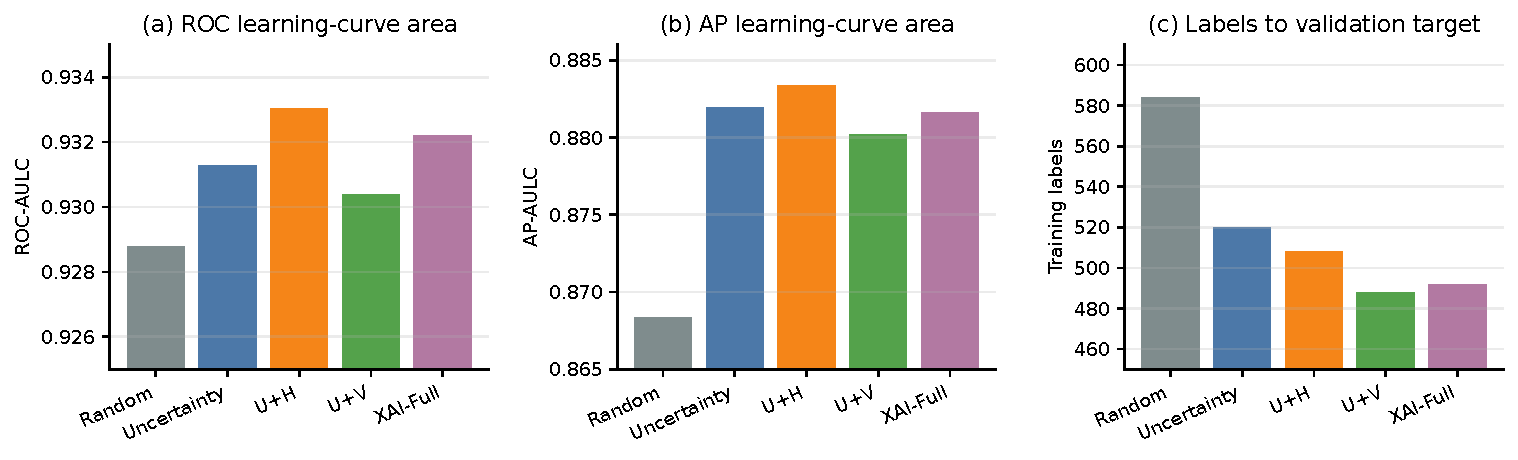
\includegraphics[width=0.93\textwidth]{al_summary.pdf}
\caption{Confirmatory active-learning summaries. Higher AULC is better; fewer
training labels to the predeclared validation target are better. Error bars are
omitted because the readiness snapshot supplies aggregate means and paired fold
effects rather than the underlying fold-level vectors in this checkout.}
\label{fig:al-summary}
\end{figure*}

\begin{table}[t]
\centering
\caption{Selected paired outer-fold effects.}
\label{tab:paired-effects}
\scriptsize
\setlength{\tabcolsep}{2.5pt}
\begin{tabular}{lrrc}
\toprule
Comparison & $\Delta$ROC & $\Delta$AP & Folds \\
\midrule
$U+H$ vs. Random & +0.004249 & +0.014985 & 5/5 \\
$U+H$ vs. Uncertainty & +0.001754 & +0.001401 & 4/5 \\
\xfull vs. Random & +0.003425 & +0.013287 & 5/5 \\
\xfull vs. Uncertainty & +0.000931 & $-0.000297$ & 3/5 \\
\bottomrule
\end{tabular}
\end{table}

Table~\ref{tab:paired-effects} makes the strongest limitation explicit.
$\xfull$ improved ROC-AULC only in three of five fold comparisons against
Uncertainty, and its mean AP-AULC difference was slightly negative. The
three-signal combination is thus not an empirically universal winner. The clearest
evidence for explanation-derived acquisition comes from $U+H$ relative to Random
and, more modestly, relative to Uncertainty.

\subsection{RQ2: Low-FPR Behavior and Computation}

Table~\ref{tab:low-fpr} reports normalized partial-AUC and TPR learning-curve
summaries. All explanation-guided methods improve substantially over Random.
Against Uncertainty, however, differences are small and change sign. Uncertainty
has the highest pAUC at FPR$\leq5\%$ and TPR-AULC at the 1\% cap; $\xfull$ is
highest at the 5\% cap. $U+H$ is slightly below Uncertainty at the 1\% cap and
slightly above it at 5\%.

\begin{table*}[t]
\centering
\caption{Learning-curve summaries in restricted false-positive regions. These are not deployment estimates at FPR $10^{-3}$ or below.}
\label{tab:low-fpr}
\small
\begin{tabular}{lccc}
\toprule
Policy & pAUC, FPR$\leq5\%$ & TPR-AULC, FPR cap 1\% & TPR-AULC, FPR cap 5\% \\
\midrule
Random & 0.804096 & 0.580620 & 0.731980 \\
Uncertainty & \textbf{0.826300} & \textbf{0.638180} & 0.769260 \\
$U+H$ & 0.824774 & 0.636780 & 0.770620 \\
$U+V$ & 0.825194 & 0.626260 & 0.768140 \\
\xfull & 0.823525 & 0.631860 & \textbf{0.771460} \\
\bottomrule
\end{tabular}
\end{table*}

The operating-region result changes the practical interpretation. Explanation
signals improve sample efficiency relative to random annotation, but the retained
study does not establish lower alert burden than a well-implemented uncertainty
baseline. Each outer test fold contains only about 300 benign samples. One false
positive therefore changes FPR by roughly 0.33 percentage points, making much
lower operational regions unresolvable.

Explanation scoring increases computation. $U+H$ adds approximately 0.227~s of
query processing across ten rounds relative to Uncertainty and increases total
model-plus-query time by 7.93\%. $\xfull$ increases the total by 4.86\%; query
processing constitutes about 5.42\% of its reported model-plus-query time. These
small absolute values apply to a 2,000-sample experiment and exclude annotation,
data loading outside the timed scope, and endpoint detection latency.

RQ2 therefore has no single optimal policy. $U+H$ is preferred when integrated
ranking quality is primary, $U+V$ when target attainment under the measured rule
is primary, and Uncertainty remains competitive in the low-FPR summaries while
avoiding TreeSHAP overhead.

\subsection{RQ3: Controlled Deletion}

Table~\ref{tab:deletion} reports AUC decreases averaged over the retained fidelity
models. Under both replacement baselines, top-$|\mathrm{SHAP}|$ deletion has a
large, monotonic effect as $k$ increases, whereas uniform random deletion has a
near-zero mean effect. For mean replacement, the top-minus-random difference is
0.047617 at $k=10$, 0.135323 at $k=25$, and 0.305750 at $k=50$. Median
replacement yields comparable differences of 0.053388, 0.124854, and 0.300119.

\begin{table*}[t]
\centering
\caption{Controlled feature-space deletion across 25 fitted models. Values are ROC--AUC decreases from the corresponding unmasked model.}
\label{tab:deletion}
\small
\begin{tabular}{lrrrr}
\toprule
Replacement & $k$ & Top-SHAP drop & Random drop & Top minus random \\
\midrule
Mean & 10 & 0.047817 & 0.000200 & 0.047617 \\
Mean & 25 & 0.135853 & 0.000530 & 0.135323 \\
Mean & 50 & 0.306729 & 0.000979 & 0.305750 \\
Median & 10 & 0.053483 & 0.000094 & 0.053388 \\
Median & 25 & 0.125180 & 0.000326 & 0.124854 \\
Median & 50 & 0.300777 & 0.000658 & 0.300119 \\
\bottomrule
\end{tabular}
\end{table*}

\begin{figure}[t]
\centering
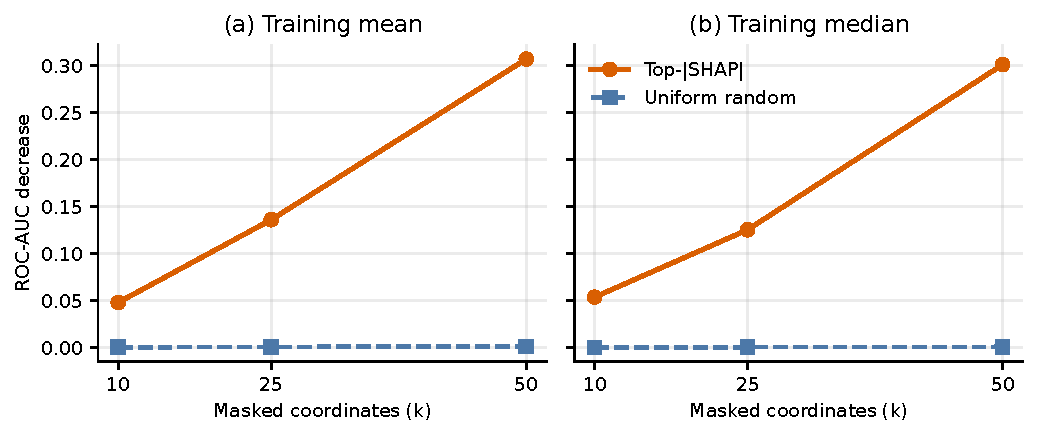
\includegraphics[width=\linewidth]{fidelity_deletion_confirmatory.pdf}
\caption{ROC--AUC decrease under top-$|\mathrm{SHAP}|$ and uniform random
replacement. Absolute effects are emphasized because ratios are unstable when
the random-control decrease is near zero.}
\label{fig:deletion}
\end{figure}

Figure~\ref{fig:deletion} shows that the result is not specific to mean
replacement. It establishes relative fitted-model reliance under both tested
training-derived baselines. Equal coordinate count does not match perturbation
magnitude or ensure that random coordinates participate in the trees; the result
should therefore not be called an executable-level fidelity certificate.

\subsection{RQ3: Attribution-Rank Stability}

Table~\ref{tab:stability} separates model-seed and fold changes. Within a fixed
fold, global Spearman agreement is 0.6144; top-10 Jaccard agreement is 0.6221 and
decreases to 0.4901 at top 50. Across folds, Spearman agreement falls to 0.5512,
and top-k Jaccard values range from 0.4416 to about 0.30.

\begin{table}[t]
\centering
\caption{TreeSHAP ranking stability.}
\label{tab:stability}
\scriptsize
\begin{tabular}{lrrrr}
\toprule
Comparison & $\rho$ & $J_{10}$ & $J_{25}$ & $J_{50}$ \\
\midrule
Seed, same fold & 0.6144 & 0.6221 & 0.5398 & 0.4901 \\
Different fold & 0.5512 & 0.4416 & 0.3073 & 0.3020 \\
\bottomrule
\end{tabular}
\end{table}

\begin{figure}[t]
\centering
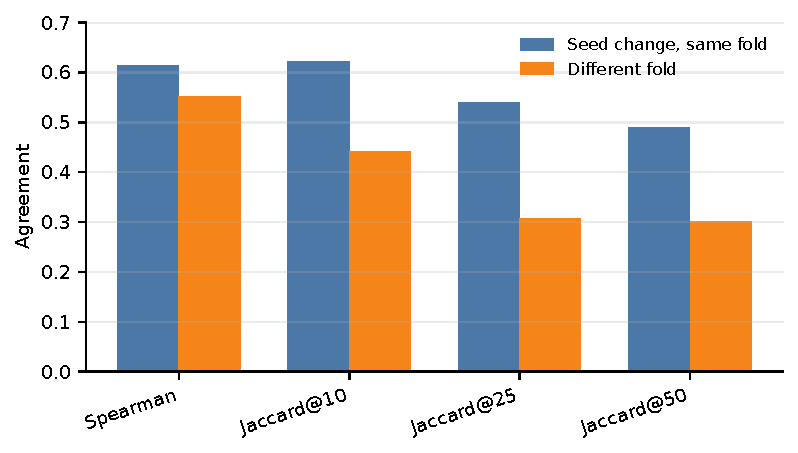
\includegraphics[width=\linewidth]{shap_stability_confirmatory.pdf}
\caption{Global and top-k agreement. Fold changes alter the learned attribution
ranking more than seed changes within a fixed fold.}
\label{fig:stability}
\end{figure}

The rankings are neither arbitrary nor invariant. They exhibit moderate
agreement, with data partitioning exerting more influence than controlled model
randomness. This finding is important for use in acquisition: a sample's
explanation-derived score follows the current fitted model and data partition,
not a stable domain truth.

Mean EC was $0.4268\pm0.0363$, and mean CF was
$0.4680\pm0.0465$ over 25 models. Mean maximum TreeSHAP additivity error was
approximately $6.0\times10^{-15}$. We treat EC and CF as descriptive geometry and
additivity as a numerical check; none of them establishes semantic correctness.


\section{Discussion}
\label{sec:discussion}

\subsection{What the Acquisition Result Means}

The clearest result is not that explanation guidance replaces uncertainty. It is
that directional attribution balance adds a small, repeatable improvement to the
learning trajectory over random acquisition and a smaller improvement over
uncertainty in four of five outer folds. $H$ distinguishes cases in which the
same output margin arises from opposing signed masses. Such cases can expose a
model boundary supported by competing PE attributes, making them plausible
queries for label acquisition.

The algebraic identity in (\ref{eq:h-identity}) also limits this interpretation.
$H$ is determined by the raw-score contribution and the $L_1$ attribution norm.
Likewise, $V$ is determined by $L_2$ magnitude and the mean signed contribution.
A direct margin-plus-norm score may recover part of the measured gain. Until
those controls are run, the result supports the tested summaries but does not
show that entropy and variance are uniquely necessary.

No policy dominates every objective. $U+H$ leads AULC, $U+V$ reaches the target
with the fewest labels, $\xfull$ performs between them, and Uncertainty remains
strong in restricted-FPR metrics. This is scientifically more informative than a
single winner: acquisition policy should be selected against an explicit
objective and operating region. A system that values early target attainment may
prefer $U+V$, whereas one that values average ranking quality throughout model
development may prefer $U+H$.

The target-based label result must also include its accounting boundary. The
numbers count labels admitted to model training. Validation labels, the full-pool
reference, dataset labeling, and analyst adjudication are additional resources.
A 92-label reduction does not imply a measured reduction in analyst hours.

\subsection{Batch Diversity and Robust Scaling}

The top-100 selection rule can query redundant samples. This risk is material
because the batch equals half of the 200-sample initial set. Uncertainty plus
k-center selection would test whether the observed gain comes from SHAP signals
or whether coverage of the same uncertain region is sufficient. A calibrated
committee would test whether ensemble disagreement explains the benefit.

Min--max normalization is also pool dependent. One extreme $H$ or $V$ value can
compress the remaining component scores and change the effective mixture.
Weight sensitivity, percentile/rank normalization, and robust quantile scaling
should be frozen and evaluated before final submission. These studies must use
validation or a nested design; selecting the best transformation from test AULC
would invalidate the outer comparison.

\subsection{What Controlled Deletion Establishes}

Top-SHAP replacement consistently damages fitted-model ranking more than
uniform random replacement at the same coordinate count, and the result holds
for mean and median baselines. This supports a relative model-reliance claim:
TreeSHAP ranks coordinates that influence these fitted LightGBM models under the
defined intervention.

Several alternatives remain. Tree ensembles use only a subset of the 2,381
coordinates; uniform random masks will often select inactive features.
Top-ranked coordinates can also lie farther from their replacement baselines,
creating a larger perturbation magnitude and greater distribution shift. A
stronger suite would select random controls from model-used features, match
absolute standardized displacement, replace semantically coupled feature
groups, and compare TreeSHAP with gain/permutation rankings.

An attribution-column permutation is a particularly useful negative control. A
common permutation preserves attribution sums, cosine similarities, centroid
distances, and norms, so additivity, EC, and CF can all remain unchanged while
feature identities are wrong. A valid identity-sensitive pipeline should fail
that control. Until it is included, EC and CF are geometry descriptions rather
than explanation certificates.

\subsection{Stability and Model Maintenance}

Moderate within-fold agreement suggests that global attribution summaries are
not dominated by model randomness. The larger reduction across folds shows that
the learned explanation depends materially on the sampled data. This matters for
model maintenance: a global top-feature list should be versioned with the model
and training cohort instead of presented as a timeless malware signature.

The active-learning use of SHAP is local and round specific, so some adaptation
of the acquisition ranking is expected. Nevertheless, a deployment study should
track rank drift, query composition, and class yield across releases. Sharp
changes can signal data drift, feature-extractor changes, or instability that
requires investigation before analyst queries are trusted.

\subsection{Relationship to Multi-Stage Fusion}

The broader thesis studies conditional static/dynamic analysis. A separate
199-sample pilot reported complementary static and API-sequence scores and found
that proportional fusion had the highest mean AUC/AP among seven configurations.
The PI and PID variants produced identical final decisions; the derivative term
added no measurable benefit at 5--20 event prefixes, and the PID-versus-fixed AUC
interval crossed zero. Those results motivate evidence-driven simplification,
not a full PID superiority claim.

That pilot uses MalBehavD-V1, logistic scorers, and event-indexed API prefixes;
the present AL/Fidelity study uses static EMBER vectors and LightGBM. Their
metrics cannot be combined into an end-to-end system result. Multi-stage
integration requires one paired cohort, a gate with final decisions for all
traffic, fixed/learned fusion baselines, and a factorial acquisition--fusion
study. We therefore keep fusion outside the contributions and abstract of this
paper.

\subsection{Practical Implications}

The most immediate use is a model-development workflow. Train a static PE model,
score a candidate pool, apply a policy chosen for the development objective,
present the selected rows to an authorized analyst, and retain query/model
lineage. Controlled deletion and stability checks can run as release diagnostics
for candidate models. They do not authorize automated remediation or substitute
for malware-analysis containment and labeling governance.

The query-computation overhead is modest in the measured small pool, but scaling
TreeSHAP to large corpora can become material. A production design may prefilter
by uncertainty and calculate explanations only for a candidate band, or cache
tree contributions for repeated policy comparisons. Such engineering changes
must be re-evaluated because they change the acquisition population.


\section{Threats to Validity}
\label{sec:threats}

\subsection{Construct Validity}

The label denotes generic benign/malware status, not ransomware. SHA-256 identity
and source-index linkage improve traceability but cannot create absent family or
behavior semantics. We therefore avoid ransomware, zero-day, and behavioral
claims.

$H$ is entropy of signed attribution mass, and $V$ is variance across one
attribution vector. Neither is calibrated model uncertainty. The term
``explanation-guided'' refers to how the signals are computed, not proof that they
encode human-understandable malware mechanisms.

Deletion measures model behavior under feature replacement. It does not establish
valid PE edits, causality, robustness to every perturbation, or human usefulness.
EC, CF, and additivity examine different constructs and are not combined into an
OFS.

\subsection{Internal Validity}

Outer test partitions are excluded from query and target selection according to
the retained protocol. Policies share initial sets within fold/seed, limiting
confounding by starting labels. The fixed policy weights and min--max
normalization, however, were not evaluated through an independent outer
sensitivity study. The measured comparison may depend on those design choices.

The oracle reveals existing labels without error. Real analysts can abstain,
disagree, or use different evidence, changing both label quality and cost. Batch
selection has no diversity constraint and may contain redundant samples.

Mean/median baselines are calculated from training data, avoiding direct test
leakage. Yet top-SHAP and random masks are not matched by displacement magnitude,
used-feature status, or manifold distance. These confounders can contribute to
the deletion gap.

\subsection{Statistical Conclusion Validity}

Five seed trajectories are averaged within each of five outer folds. The paired
outer fold is the comparison unit; fold--seed combinations are not 25 independent
test datasets. Five folds support effect-size and direction reporting but limited
formal inference. The readiness snapshot does not provide fold-level vectors in
this checkout, so figures assembled here omit uncertainty bars. The submission
artifact must regenerate them directly from retained fold-level files.

Twenty random masks per $k$ characterize mask variability conditional on each
fitted model. The 25 fidelity models share data and folds, so model-level records
are also dependent. Pairwise rank comparisons share models and cannot be counted
as independent observations in a naive significance test.

Restricted-FPR estimates use small outer test folds. With roughly 300 benign
rows, one false positive changes FPR by about 0.33 percentage points. Results at
1\% and 5\% caps do not validate operation at $10^{-3}$ or $10^{-4}$.

\subsection{External Validity}

The 2,000 rows form a short-period subset recovered from EMBER material and do
not reproduce the full official benchmark protocol. Random row folds do not
enforce temporal, family, source, or campaign separation. Results may change
under newer software, another organization, a different benign distribution,
another feature extractor, or adversarial manipulation. External and temporal
validation are required for a broad journal claim.

LightGBM and TreeSHAP are central to the experiment. The acquisition statistics
can be defined for other additive attributions, but their numeric behavior,
cost, and stability may differ for raw-byte networks, graph models, or sequence
models.

\subsection{Reproducibility Validity}

The readiness report names source commit
\texttt{fed4322f58f5bb55ec47833e857370d076592a32}, locked dataset/manifest hashes,
and replay counts. That commit and the confirmatory result directory are not
available in the cloud checkout used for this manuscript revision. We therefore
attribute numerical values to the retained readiness report and do not describe
this writing pass as an independent rerun. Before submission, the exact source
and artifacts must be synchronized, hashes verified, replay executed in a clean
environment, and all tables/figures regenerated from source records.

Computational replay establishes consistency with stored data and code. It does
not prove external label correctness, data-sharing rights, or generalization.

\section{Conclusion}
\label{sec:conclusion}

This paper evaluated explanation-guided active learning and controlled TreeSHAP
diagnostics for static Windows PE malware classification. The acquisition family
combines predictive uncertainty with directional entropy and signed-attribution
variance. On an identity-audited 2,000-sample EMBER subset, evaluated with five
outer folds and five seeds per fold, $U+H$ achieved the highest ROC/AP learning-
curve area. Its improvements over Random were positive in every outer fold;
improvements over Uncertainty were smaller and occurred in four of five folds.
$U+V$ reached the predeclared validation target with the fewest mean training
labels, while $\xfull$ reduced the mean budget by 92 labels relative to Random.
No configuration was best across learning quality, target attainment, restricted-
FPR behavior, and computation.

The TreeSHAP study extended the evaluation to 25 fitted models. Top-ranked
coordinates produced substantially larger AUC decreases than equal-count random
coordinates under both training-mean and training-median replacement. Global and
top-k rankings showed moderate agreement and were less stable across data folds
than across seeds within one fold. These findings support relative reliance of
the fitted models on the ranked coordinates under the specified interventions.
They do not establish causal malware features or valid executable edits.

The results motivate a focused next experiment rather than a broader deployment
claim. Uncertainty plus diversity, calibrated committee acquisition, weight and
normalization sensitivity, stronger deletion controls, and external/temporal
evaluation are the primary evidence gates. Completing them would determine
whether the measured gains reflect uniquely useful explanation signals and
whether they transfer beyond the audited subset.

The study also illustrates a general reporting principle for security ML: label
efficiency, operating-point quality, attribution behavior, and reproducibility
answer different questions. Reporting their trade-offs and limitations provides
a stronger basis for model maintenance than selecting a single favorable AUC or
explanation image.



\appendices
\section{Active-Learning Replay Checklist}
\label{app:al}

For each outer fold and AL seed, a reproducible run should retain:

\begin{enumerate}
    \item development, validation, and test row identifiers;
    \item the shared 200-row initial labeled set and ordered remaining pool;
    \item model configuration, library versions, and all deterministic seeds;
    \item validation/test probabilities and labels for every round;
    \item pool probabilities, $U/H/V$ components, normalized values, composite
    scores, ranks, and queried row identifiers;
    \item the full-pool validation reference and target calculation;
    \item per-round ROC--AUC, AP, low-FPR summaries, and scoped timings;
    \item saved checkpoints or a deterministic reconstruction mechanism;
    \item verification output confirming query membership, uniqueness, no
    test/validation leakage, additivity, and metric recomputation.
\end{enumerate}

Every policy within a fold/seed must begin from the same initial set. The test
partition must remain unavailable to query selection, target construction,
weight selection, threshold selection, and stopping.

\section{Fidelity Replay Checklist}
\label{app:fidelity}

For every outer fold and model seed:

\begin{enumerate}
    \item retain the fitted model, split IDs, training mean and median, and raw
    TreeSHAP matrix including the bias separately;
    \item verify raw-score additivity before ranking features;
    \item save top-$k$ and random mask indices for every sample, $k$, control
    draw, and replacement baseline;
    \item reconstruct masked matrices from the original test vectors and saved
    indices rather than from plotted summaries;
    \item retain original/masked probabilities and recompute AUC decreases;
    \item retain global rankings and model-pair identifiers used for Spearman and
    Jaccard summaries;
    \item label EC and CF as geometry diagnostics and confirm that no composite
    OFS is introduced without a preregistered rule.
\end{enumerate}

Future controls should include random selection restricted to model-used
features, matched standardized displacement, attribution-column permutation, and
schema-aware group replacement.

\section{Interpretation Boundaries}

\begin{table*}[h]
\centering
\caption{What the reported quantities establish and do not establish.}
\label{tab:boundaries}
\scriptsize
\setlength{\tabcolsep}{3pt}
\begin{tabular}{p{2.4cm}p{5.8cm}p{6.5cm}}
\toprule
Quantity & Supported interpretation & Unsupported interpretation \\
\midrule
ROC/AP-AULC & Ranking quality integrated over the measured label budgets & Analyst labor, calibration, or external generalization \\
Labels to target & Training labels to a fold-specific validation target & Total annotation cost or hours saved \\
Low-FPR summaries & Relative performance at 1\%/5\% caps in the outer folds & Reliable FPR at $10^{-3}$ or $10^{-4}$ \\
$H$ & Balance of positive/negative TreeSHAP mass & Predictive entropy or causal conflict \\
$V$ & Dispersion across signed attribution coordinates & Ensemble or posterior uncertainty \\
Top-k deletion & Fitted-model sensitivity under training-statistic replacement & Valid PE transformation or causal malware mechanism \\
Additivity & Numerical reconstruction of the raw tree score & Correct feature identity or human usefulness \\
EC/CF & Geometry of retained attribution vectors & Explanation correctness certificate \\
Seed/fold agreement & Sensitivity to fitted model and data split & Stability across organizations and time \\
Replay verification & Consistency with retained code/data/artifacts & Independent external replication or data authenticity \\
\bottomrule
\end{tabular}
\end{table*}

\section{Claim--Evidence Map}

\begin{table*}[h]
\centering
\caption{Central claims and submission status.}
\label{tab:claims}
\scriptsize
\begin{tabular}{p{5.2cm}p{3.0cm}p{6.9cm}}
\toprule
Claim & Status & Scope or required wording \\
\midrule
$U+H$ exceeds Random in ROC/AP-AULC & Reported supported & Five outer folds; report paired effect and direction \\
$U+H$ universally exceeds Uncertainty & Not supported & Small effects; favorable in 4/5 folds \\
\xfull saves 92 training labels vs. Random & Reported supported & Validation labels/reference cost are additional \\
\xfull is the best policy & Not supported & $U+H$ leads AULC; $U+V$ uses the fewest labels \\
Top-SHAP deletion exceeds random deletion & Reported supported & Feature space; 25 models; mean/median; absolute effects \\
TreeSHAP identifies causal malware features & Not supported & No executable-valid or causal intervention \\
Rankings are invariant & Not supported & Moderate agreement; lower across folds \\
The study detects ransomware/zero-day families & Not supported & Generic PE malware labels only \\
The cloud revision independently replayed results & Pending & Synchronize named source/artifacts and rerun verification \\
\bottomrule
\end{tabular}
\end{table*}

\section{Pre-Submission Evidence Gates}

The following items should be completed before journal submission:

\begin{enumerate}
    \item synchronize commit
    \texttt{fed4322f58f5bb55ec47833e857370d076592a32} and the complete confirmatory
    result directory; verify the locked dataset and manifest hashes;
    \item rerun the verification entry point in a clean environment and generate
    every table/figure directly from retained fold-level data;
    \item add uncertainty-plus-diversity and a calibrated committee baseline;
    \item add weight/normalization sensitivity and batch-redundancy analysis;
    \item add identity-sensitive and magnitude-matched fidelity controls;
    \item obtain external, temporal, or source-disjoint evidence if the target
    venue expects broad generalization;
    \item verify bibliography metadata against publisher records and confirm
    authorship, ORCID, corresponding author, data rights, and the current journal
    template.
\end{enumerate}

\clearpage

\bibliographystyle{IEEEtran}
\bibliography{references}
\end{document}
